%%%%%%%% ICML 2027 SUBMISSION (built on the icml2026 style; swap the style
%%%%%%%% file for icml2027 when the official kit is released — one line).
\documentclass{article}

\usepackage{microtype}
\usepackage{graphicx}
\usepackage{booktabs}
\usepackage{xcolor}

% Submission mode (anonymous, line numbers). Camera-ready: [accepted].
\usepackage{icml2026}

\usepackage{amsmath}
\usepackage{amssymb}
\usepackage{mathtools}
\usepackage{amsthm}
\usepackage[capitalize,noabbrev]{cleveref}

% ---- pending-experiment marker: every stub is visible and greppable ----
\newcommand{\pending}[1]{\textcolor{purple!80!black}{\textbf{[Pending:} #1\textbf{]}}}

% ---- per-section takeaway box ----
\definecolor{shadecolor}{gray}{0.94}
\newsavebox{\takeawaybox}
\newenvironment{takeaway}%
{\begin{lrbox}{\takeawaybox}\begin{minipage}{\dimexpr\columnwidth-14pt}%
\small\textbf{Takeaway.}\ }%
{\end{minipage}\end{lrbox}\par\vspace{4pt}\noindent%
{\setlength{\fboxsep}{6pt}\colorbox{shadecolor}{\usebox{\takeawaybox}}}\par\vspace{4pt}}
\newcommand{\cmark}{\checkmark}
\newcommand{\xmark}{$\times$}

\icmltitlerunning{Novelty-Gated Compensation in a VLA Policy}

\begin{document}

\twocolumn[
\icmltitle{Novelty-Gated Compensation: What Causally Hijacking Actions\\
Reveals About Self-Attribution in VLA Policies}
% Alt titles:
% "The Policy Reacts to What It Sees, Not What It Did"
% "The Comparison Is Cheap and the Policy Never Buys It"

\icmlsetsymbol{equal}{*}

\begin{icmlauthorlist}
\icmlauthor{Anonymous Authors}{anon}
\end{icmlauthorlist}

\icmlaffiliation{anon}{Anonymous Institution}
\icmlcorrespondingauthor{Anonymous}{anon@anon.org}

\icmlkeywords{vision-language-action, world models, interpretability, probing, causal intervention}

\vskip 0.3in
]

\printAffiliationsAndNotice{}

\begin{abstract}
Do learned robot policies internalize their own causal role in the world, or
do they merely predict from what they see? We adjudicate with a causal
audit: during closed-loop rollouts of 7B vision--language--action policies
(OpenVLA-OFT) on four LIBERO suites, we covertly hijack the executed action
chunk with probability $0.25$ and ask whether anything inside the policy
distinguishes self-caused from hijacked transitions. Across seven runs---a
discovery run, a pre-registered seed replication, three further suites with
their own checkpoints, and two gross-violation arms---no hidden-state probe,
linear or one-hidden-layer MLP, separates from a selection-matched
shuffled-label floor wherever the executed outcome is kinematically
plausible. The null carries its own positive controls. Comparison features
of command and outcome decode the same label at $0.69$--$0.91$ in every run;
a 256-unit MLP handed only the raw command$\,\oplus\,$outcome concatenation
\emph{computes} the comparison ($0.69$ vs.\ $0.46$ for its linear
counterpart)---swap the outcome half for hidden states and decoding
collapses to floor. The ingredients are present (the commanded plan reads
out of the pre-action state at $R^2{=}0.64$, replicating at the same layer
and pool), and the computation is demonstrably cheap; the policy's states
never expose it. The policy does react behaviorally---but the reaction is
gated by the \emph{visual novelty} of the outcome, not by the decodable
command--outcome mismatch: significant after visibly reversed motion
($p{\approx}0.01$, $n{=}119$ episodes), absent after the mechanically most
blatant intervention, freezing ($n{=}115$), and small and seed-fragile for
stealthy swaps (significant in 2 of 5 arms; null in the pre-registered
replication). We call this \emph{novelty-gated compensation}: the policy
corrects what it sees without representing what it did. The audit costs
under 5 GPU-hours end to end, and we report every pre-registered verdict,
including the one that went against us.
\end{abstract}

\section{Introduction}
\label{sec:intro}

When an animal acts, its nervous system routes a copy of the outgoing motor
command---an \emph{efference copy}---into sensory processing, letting it
distinguish ``the world changed because I moved'' from ``the world changed on
its own''~\citep{vonholst1950,sperry1950,crapse2008}. Whether learned robot
policies contain anything analogous has become a live fault line. One line of
work reads rich \emph{world models} into sequence models and policies:
internal representations of state, dynamics, and consequences
\citep{ha2018world,hafner2020dream,li2023othello,gurnee2024language}, an
assumption made operational by pipelines that train policies inside learned
action-conditioned world models \citep{zhu2025wmpo}. A second line documents
\emph{action-blindness}: predictive representations that keep improving while
becoming insensitive to the agent's own causal contribution
\citep{li2026dueling}, and minimal agents that behaviorally compensate for
hijacked actions without encoding the self/other distinction anywhere
\citep{ye2026prediction}. Self-vs.-external attribution is the sharpest point
of contact between these accounts, so we pose it as a measurement:

\begin{center}
\emph{When an executed action was not the policy's own, does anything
inside the policy register that fact?}
\end{center}

We answer causally. During closed-loop rollouts of OpenVLA-OFT
\citep{kim2025oft} on the LIBERO suites \citep{liu2023libero}, we covertly
replace the executed action chunk with probability $0.25$---primarily by
\emph{swapping in another same-task episode's chunk}, so that executed
actions keep natural task statistics---and ask three pre-registered
questions. (\textbf{Q1}) Does the post-hijack hidden state carry a readable
trace that the transition was externally imposed? (\textbf{Q2}) If a probe
is handed the missing efference---the commanded chunk, or both pre- and
post-action states---does attribution become easy; i.e., is the
representation \emph{format} such that an efference comparison would be
cheap if one were ever performed? (\textbf{Q3}) Does the policy react
behaviorally regardless, and to what signal?

One architectural fact sharpens the design: these checkpoints are memoryless
and vision-only per call (one third-person image plus the instruction; no
proprioception, no action history), so the policy \emph{cannot} literally
compare its previous command to the observed outcome---Q1 and Q2 ask whether
its representation nevertheless supports the comparison, and Q3 asks what
its closed-loop behavior does instead.

\begin{figure*}[t]
\centering
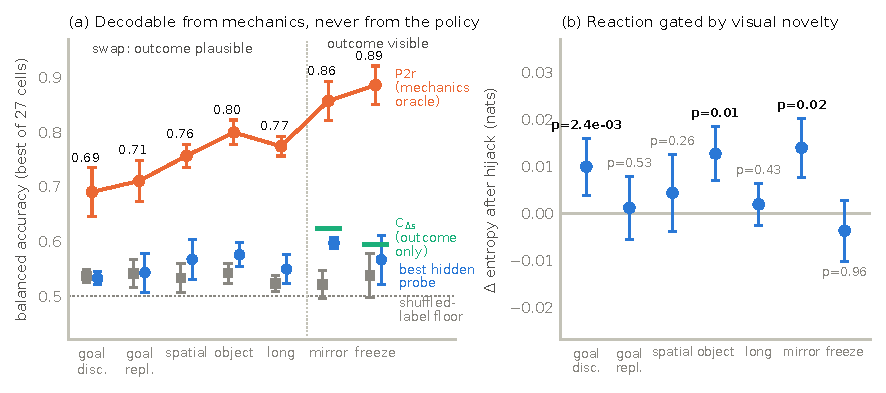
\includegraphics[width=\textwidth]{fig_headline.pdf}
\caption{\textbf{The dissociation across seven runs.} \textbf{(a)}~Best-cell
balanced accuracy per run (linear family; error bars: fold sd). The
mechanics oracle P2r (comparison features of commanded chunk vs.\ observed
state change) decodes the hijack label in every run ($0.69$--$0.89$), while
the best hidden-state probe tracks each run's selection-aware shuffled-label
floor in all five \textsc{swap} arms; in \textsc{mirror}/\textsc{freeze} it
rises exactly as far as the visible-outcome control C$_{\Delta s}$ (short
dashes) allows---the outcome is \emph{seen}, not attributed
(\cref{sec:results-visible}). \textbf{(b)}~Next-call entropy shift after a
hijack vs.\ phase-matched self transitions ($\pm1$\,SE over episodes;
episode-level Wilcoxon $p$, bold $=$ significant). The reaction follows
visual novelty (\textsc{mirror}), not mechanical decodability
(\textsc{freeze}, the most decodable and least reactive); for stealthy
\textsc{swap}s it is small and inconsistent across runs (2 of 5
significant).}
\label{fig:headline}
\end{figure*}

The answers dissociate (\cref{fig:headline}). \emph{Attribution is not
readable.} Across five swap runs---two seeds on LIBERO-Goal and one run each
on Spatial, Object, and Long, each suite with its own SFT
checkpoint---no probe on hidden states separates from a selection-aware
shuffled-label floor: not given the post-hijack state alone, not given the
commanded chunk as well, not given both pre- and post-action states, and not
when the probe family is upgraded from logistic regression to one-hidden-layer
MLPs (\cref{sec:results-attr}). The null comes with unusual internal support.
In the same data, explicit command--outcome comparison features decode the
label at $0.690$--$0.911$; the policy's own 56-dimensional motor plan reads
out of its pre-action state at $R^2{=}0.639$, replicating at $0.638$ at the
same layer and pool on a fresh seed; and---the sharpest control---the same
MLP family that finds nothing in hidden states \emph{computes the comparison
itself} when handed the raw mechanical ingredients ($0.687$ vs.\ a $0.463$
linear baseline on the identical feature blocks). The ingredients are
present and the computation is cheap; it is the policy's representation that
never exposes it.

\emph{Yet the policy is not indifferent.} One call after a hijack its action
distribution shifts---but the shift follows what the outcome \emph{looks}
like, not how badly execution betrayed the command. Visibly reversed motion
(\textsc{mirror}) provokes it ($p{=}0.016$/$0.012$ at $n{=}119$ episodes);
a frozen arm---the mechanically most decodable intervention (P2r
$0.886$--$0.911$) but a visually unremarkable one---provokes nothing
($n{=}115$, both metrics wrong-signed); kinematically plausible
\textsc{swap}s sit at the detection threshold, significant in 2 of 5 runs
and null in the pre-registered replication (\cref{sec:results-novelty}). We
name this \textbf{novelty-gated compensation}: closed-loop correction driven
by how unusual the observation looks, with no readable representation of
whose action caused it.

\textbf{Contributions.}
\textbf{(1)}~\emph{The Hijack--Probe protocol} (\cref{sec:protocol}): a
causal audit for self-attribution in embodied policies combining covert
action hijacking, verified hidden-state capture, selection-aware nulls for
two probe families, phase-matched negatives, and mechanical positive
controls---to our knowledge the first instrument that makes ``does the
policy know what it did?'' a measured quantity rather than a narrative
(\cref{tab:taxonomy}).
\textbf{(2)}~\emph{An adjudication with receipts} (\cref{sec:results-attr}):
for 7B SFT-trained VLAs the action-blind account wins at the level of
readable representation---replicated across seeds, generalized across four
suites and checkpoints, and robust to the probe-family upgrade---even though
the world-model account is right that the motor plan is linearly present.
\textbf{(3)}~\emph{A capacity argument} (\cref{sec:results-cheap}): holding
family, samples, and command features fixed, a one-hidden-layer MLP computes
the self/other comparison from raw command$\,\oplus\,$outcome ingredients
but not from any probed hidden state; absence in the states is therefore not
explained by the comparison being hard.
\textbf{(4)}~\emph{A mechanism} (\cref{sec:results-novelty}):
novelty-gated compensation, established by a behavioral fingerprint whose
two poles (\textsc{mirror} vs.\ \textsc{freeze}) are now each powered by
${>}110$ episodes; it extends the compensation-without-encoding dissociation
of \citet{ye2026prediction} from minimal agents to real 7B policies and
gives it a positive gating variable.
\textbf{(5)}~\emph{Calibration traps and pre-registration receipts}
(\cref{sec:traps,sec:receipts}): five ways naive versions of this experiment
return the wrong answer, and a worked example of pre-registered
interpretability---four readout rules fixed in an append-only log before the
second wave was collected, every verdict reported, including a
non-replication that costs us a claim.

\section{Positioning}
\label{sec:related}

\begin{table*}[t]
\caption{How prior work tests what is ``inside'' a policy, versus the
Hijack--Probe protocol. Each column is a property we argue is necessary for
the attribution question specifically: causal intervention separates
self-caused from external transitions on-policy; selection-aware nulls keep
best-of-$N$ probe sweeps honest; a positive control certifies the label is
recoverable at all; measuring behavior and representation on the same events
is what exposes dissociations. Representative examples: correlational probing
\citep{alain2017,li2023othello,gurnee2024language}, control tasks
\citep{hewitt2019}, action-sensitivity analyses \citep{li2026dueling},
toy-agent hijacking \citep{ye2026prediction}.}
\label{tab:taxonomy}
\vskip 0.1in
\centering
\footnotesize
\begin{tabular}{lcccc}
\toprule
Approach & \shortstack{Causal\\intervention} & \shortstack{Selection-aware\\null} & \shortstack{Positive\\control} & \shortstack{Behavior $+$\\representation} \\
\midrule
Behavioral evaluation (success rates) & \xmark & --- & \xmark & \xmark \\
Correlational probing of policies/LLMs & \xmark & rare & rare & \xmark \\
Action-sensitivity analyses of world models & \cmark & \xmark & \xmark & \xmark \\
Toy-agent hijacking & \cmark & \xmark & \xmark & \cmark \\
\textbf{Hijack--Probe (ours)} & \cmark & \cmark & \cmark & \cmark \\
\bottomrule
\end{tabular}
\vskip -0.1in
\end{table*}

\textbf{Efference copies and corollary discharge.} The reafference principle
\citep{vonholst1950} and corollary discharge \citep{sperry1950} describe
circuitry that predicts and cancels the sensory consequences of
self-generated action; \citet{crapse2008} review its ubiquity across taxa. We
import the concept as a representational hypothesis about artificial
policies, not as a claim about biological similarity.

\textbf{World models inside networks.} Evidence that sequence models
internalize latent structure ranges from game-board state
\citep{li2023othello} to geographic and temporal structure
\citep{gurnee2024language}; in robotics, world models are trained explicitly
for control \citep{ha2018world,hafner2020dream} and, recently, as
environments for on-policy RL of VLAs \citep{zhu2025wmpo}. All of these
presuppose that action information enters the learned dynamics.

\textbf{Action-blindness and compensation without encoding.}
\citet{li2026dueling} show latent world models can go action-blind:
predictions for different actions become indistinguishable while training
loss improves. \citet{ye2026prediction} construct minimal agents that
behaviorally compensate for hijacked actions without encoding agency. Our
protocol ports this intervention logic to full-scale VLAs and adds the
calibration machinery (\cref{tab:taxonomy}) that a 7B-scale null needs to be
interpretable.

\textbf{Probing methodology.} Linear probes \citep{alain2017} require
control tasks \citep{hewitt2019} and careful interpretation
\citep{belinkov2022}. We contribute a \emph{selection-aware} floor for
best-of-$N$ cell sweeps, instantiated for both probe families
(\cref{sec:protocol-probes}), without which this paper would have reported
two different false positives (\cref{sec:traps}).

\section{The Hijack--Probe Protocol}
\label{sec:protocol}

\begin{figure*}[t]
\centering
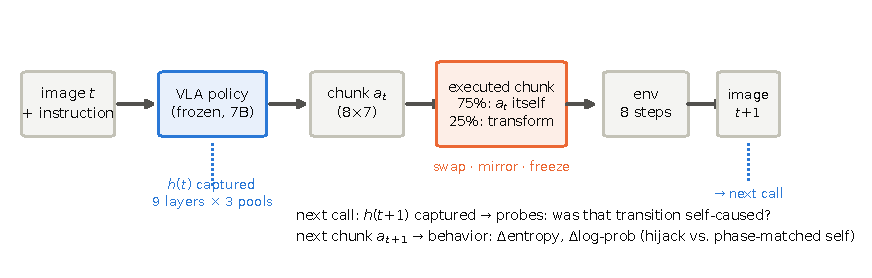
\includegraphics[width=0.94\textwidth]{fig_setup.pdf}
\caption{\textbf{The intervention loop.} The frozen policy emits an
$8\times7$ action chunk from one third-person image and the instruction.
With $p{=}0.25$ (4-call warm-up; $\geq2$ clean calls after each hijack) the
\emph{executed} chunk is replaced by a transform: \textsc{swap} (another
same-task episode's chunk), \textsc{mirror} (negated $x/y$ translation), or
\textsc{freeze} (zero motion). Hidden states are captured at 9 layers
$\times$ 3 token pools on every call.}
\label{fig:setup}
\end{figure*}

\textbf{Subjects and scale.} OpenVLA-OFT (7B), SFT per suite, evaluated at
its released stochastic sampling protocol (temperature $1.6$); no
proprioception, no wrist camera; action chunks of $K{=}8$ steps $\times$ 7
DoF. Seven runs over two waves: a \emph{discovery} run (LIBERO-Goal, all 10
tasks $\times$ 30 initial states $=$ 300 episodes), a \emph{replication} run
(same protocol, fresh seed, 200 episodes), expanded \textsc{mirror} and
\textsc{freeze} arms (150 episodes each, on the five goal tasks where
interventions perturb mechanics most), and one \textsc{swap} run on each of
LIBERO-Spatial, -Object, and -Long (200/200/150 episodes), each under that
suite's own SFT checkpoint. Totals: 1{,}350 episodes, 46{,}931 policy calls,
5{,}635 hijacks; $20$--$23\%$ of episodes per run stay entirely clean. All
collection, pilots and control arms included, cost $4.8$ GPU-hours on one
24\,GB workstation GPU; probing is CPU-only ($\approx$10\,h on 16 vCPUs for
the second wave).

\textbf{Causal hijack.} At each eligible call the executed chunk is the
policy's own (\textsc{self}) or a transform of it (\textsc{hijack}), i.i.d.\
with $p{=}0.25$ after a 4-call warm-up and never on consecutive calls, so
the state one call later reflects exactly one manipulated transition
(\cref{fig:setup}). \textsc{swap}, the primary transform, executes another
same-task episode's commanded chunk: replacements retain natural task
statistics, so a probe cannot win by detecting implausible kinematics.
\textsc{mirror} and \textsc{freeze} are gross-violation arms in which the
outcome \emph{is} visibly anomalous---by design, since they bound what
outcome perception alone can explain (\cref{sec:results-visible}).

\textbf{Verified capture.} Hidden states are recorded at layers
$\{0,4,\dots,32\}$ under three pools (context mean; last pre-action token;
mean over the 56 positions from which actions are decoded). A runtime
self-check reproduces the model's own action log-probabilities from the
captured slice (max deviation $4.8\times10^{-7}$), ruling out indexing
errors before any probe is trained.

\subsection{Probes, two families, and the selection-aware floor}
\label{sec:protocol-probes}

Each probe sample pairs consecutive calls: positives follow a hijack;
negatives follow a \textsc{self} transition \emph{from the same episode},
phase-matched by minimum-cost assignment on call index ($n{=}1{,}056$ to
$2{,}354$ balanced samples per run). Probes come in two families on the same
frozen features: $\ell_2$-regularized logistic regression, and a 256-unit
one-hidden-layer MLP (\texttt{lbfgs}, $\alpha$ grid inner-selected). Both
use 5-fold CV grouped by episode and inner-split hyperparameter selection;
\cref{tab:probes} defines the ladder. Because each probe is reported at its
best of 27 layer$\times$pool cells, comparing to $0.5$ overstates it: the
floor is the maximum over the \emph{same} 27 cells of a shuffled-label probe
(P0) \emph{of the same family}, complemented by a fixed-cell permutation
null. Floors land at $0.52$--$0.54$ across runs and families; effects below
${\approx}0.03$--$0.04$ balanced accuracy are undetectable at these $n$.

\textbf{Pre-registration.} The second wave---replication seed, expanded
arms, suite runs, the MLP family, and four readout rules---was fixed in an
append-only log before any of its data existed. \cref{sec:receipts} reports
each rule's verdict; the log ships with the code.

\begin{table}[t]
\caption{Probe ladder. $h(t)$/$h(t{+}1)$: hidden states before/after the
manipulated transition; $a$: commanded chunk; $\Delta s$: simulator state
change. Every probe is run in both families.}
\label{tab:probes}
\vskip 0.1in
\centering
\small
\setlength{\tabcolsep}{3pt}
\begin{tabular}{ll}
\toprule
Probe & Input (question) \\
\midrule
P0 & hidden state, shuffled labels (selection floor) \\
P1 & $h(t{+}1)$ \hfill (anomaly trace without efference; Q1) \\
P3 & $a \oplus h(t{+}1)$ \hfill (efference-augmented; Q2) \\
P4 & $h(t) \oplus h(t{+}1)$ \hfill (internal efference; Q2) \\
P2 & $a \oplus \Delta s$ concatenated \hfill (mechanical baseline) \\
P2r & comparison features of $(a,\Delta s)$ \hfill (oracle) \\
C$_{\text{cmd}}$/C$_{\Delta s}$/C$_{\text{ph}}$ & $a$ / $\Delta s$ / phase alone \hfill (leakage) \\
\bottomrule
\end{tabular}
\vskip -0.1in
\end{table}

\subsection{Behavioral battery}
\label{sec:protocol-behavior}

We measure, on the call immediately after each hijack vs.\ its phase-matched
\textsc{self} control: action-token entropy and chosen-chunk
log-probability (episode-level Wilcoxon signed-rank; the conservative unit),
episode success in hijack-carrying vs.\ clean episodes, and a
\emph{corrective-behavior} metric---does the next command re-assert motion
blocked by \textsc{freeze}?---reported only after replacing the next command
with its AR(1) innovation, because the raw metric is confounded by command
autocorrelation (\cref{sec:traps}).

\section{Results I: Attribution Is Not Readable---and the Null Carries Its Own Positive Controls}
\label{sec:results-attr}

\begin{figure}[t]
\centering
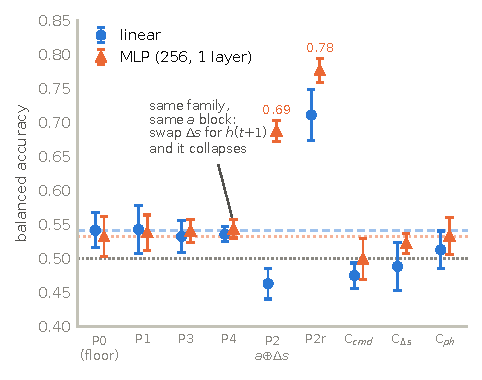
\includegraphics[width=\columnwidth]{fig_ladder.pdf}
\caption{Replication-run ladder under both probe families (best of 27
layer$\times$pool cells $\pm$ fold sd; single-cell probes as marked).
Hidden-state probes (P1/P3/P4) sit at their family's selection floor under
\emph{both} families. The mechanical rungs move: upgrading the family lifts
P2 from $0.463$ to $0.687$---the MLP computes the command--outcome
comparison that logistic regression provably cannot---and P2r from $0.711$
to $0.776$. The same upgrade does nothing for any probe whose outcome side
is a hidden state.}
\label{fig:ladder}
\end{figure}

\paragraph{The null, and its replication.}
In the discovery run, P1 $=0.525\pm0.025$, P3 $=0.525\pm0.019$, P4
$=0.533\pm0.012$: all at or below the selection floor of $0.536\pm0.011$,
leakage controls at chance, held-out-task transfer flat at $0.50$. The
pre-registered replication (fresh seed) reproduces every layer of this:
floor $0.541$, P1/P3/P4 $=0.543/0.532/0.536$, controls at chance, P2r
$0.711\pm0.038$ vs.\ $0.690\pm0.044$ (\cref{tab:replication}). Even the
readout geometry replicates: the commanded 56-dim chunk reads out of the
pre-action state at $R^2{=}0.639$ in the discovery run and $0.638$ in the
replication, \emph{at the same cell} (layer 28, action-window mean;
\cref{fig:e1}). The plan is present; the plan is stably placed; attribution
still is not.

\begin{table}[t]
\caption{The replication in one table (linear family; best cell $\pm$ fold
sd). Every quantity reproduces within fold noise; pre-registered rule (b) of
\cref{tab:receipts}.}
\label{tab:replication}
\vskip 0.1in
\centering
\small
\setlength{\tabcolsep}{3.5pt}
\begin{tabular}{lcc}
\toprule
 & disc.\ ($n{=}1716$) & repl.\ ($n{=}1266$) \\
\midrule
P0 floor & $0.536\pm0.011$ & $0.541\pm0.026$ \\
perm.\ $p_{95}$ & $0.516$ & $0.523$ \\
P1 & $0.525\pm0.025$ & $0.543\pm0.035$ \\
P3 & $0.525\pm0.019$ & $0.532\pm0.023$ \\
P4 & $0.533\pm0.012$ & $0.536\pm0.011$ \\
P2r & $0.690\pm0.044$ & $0.711\pm0.038$ \\
E1 best $R^2$ (cell) & $0.639$ (L28/act) & $0.638$ (L28/act) \\
\bottomrule
\end{tabular}
\vskip -0.1in
\end{table}

\paragraph{Upgrading the probe family does not help---except where it
should.}
\label{sec:results-cheap}
A one-hidden-layer MLP with a selection-matched MLP floor leaves the picture
unchanged on hidden states: on the replication run, P1/P3/P4
$=0.538/0.540/0.543$ against an MLP floor of $0.532$ (\cref{fig:ladder}).
By the pre-registered rule, the claim strengthens from ``no \emph{linearly}
readable trace'' to ``no readable trace, linear or one-hidden-layer MLP.''
The decisive part is what the \emph{same} family upgrade does elsewhere in
the ladder. P2---logistic regression on the raw concatenation
$a\oplus\Delta s$---sits at $0.463$, as it must: agreement between two
vectors is bilinear, not linear (\cref{sec:traps}, T2). The MLP on the
identical features reaches $0.687$ (AUROC $0.754$), nearly closing the gap
to the hand-engineered comparison oracle P2r ($0.776$), with the
$\Delta s$-only control at $0.522$: the network is computing the
comparison, not reading a marginal. Now hold the family (MLP), the command
block ($a$), the samples, and the CV fixed, and change only the outcome
block: $a\oplus\Delta s$ decodes at $0.687$; $a\oplus h(t{+}1)$---P3, with
$h(t{+}1)$ at its best of 27 cells---decodes at $0.540$, i.e.\ floor. A
256-unit MLP can perform this comparison at these sample sizes;
what it cannot do is extract the outcome side from the policy's own hidden
state. The comparison is cheap. The policy never buys it.

\paragraph{Generalization: four suites, four checkpoints.}
The same signature holds on LIBERO-Spatial, -Object, and -Long under their
own checkpoints (linear family; \cref{tab:arms-linear}): P2r $0.757/0.800/
0.774$ against floors of $0.533/0.542/0.523$, hidden rungs within
$0.022$--$0.034$ of their floors ($\leq\!1.5$ fold sd; every rung, in every
run, including both goal-suite runs, also exceeds the \emph{fixed-cell}
permutation $p_{95}$---the systematic gap between the two nulls is exactly
the selection effect of T1, which is why the selection floor is the
operative comparator). The MLP pass on Spatial reproduces its linear
picture (rungs $0.566$--$0.572$ vs.\ MLP floor $0.542$; P2 $0.769$, P2r
$0.827$). Two pre-registered MLP passes (Object, Long) were cut by a
compute budget rule fixed in the log and remain open; their linear ladders
are at floor.

\paragraph{When the outcome is visible, probes light up---exactly as far as
outcome perception allows.}
\label{sec:results-visible}
The expanded gross-violation arms are the intended stress test: after
\textsc{mirror} or \textsc{freeze}, the scene itself betrays the
intervention (the arm moved backwards; the arm did not move). Hidden-state
probes now do clear their floors---mirror P4 $0.597\pm0.011$ linear /
$0.612$ MLP; freeze P4 $0.566\pm0.045$ linear / $0.636$ MLP---and this is
not an efference signature but a \emph{sensitivity control}, for two
pre-specified reasons. First, the observable-outcome control bounds every
one of these excursions within its family: C$_{\Delta s}$ (simulator state
change alone, no hidden states, no command) decodes $0.623$/$0.738$
(mirror, linear/MLP) and $0.594$/$0.825$ (freeze), i.e.\ at least as much
label as any hidden rung, while C$_{\text{cmd}}$ stays at chance
($0.485$--$0.520$) in all four family$\times$arm combinations. What the
states carry is what the \emph{camera} carries: an unusual outcome, not its
authorship. Second, the pattern was predicted in advance from the synthetic
fixture of T2 (directed motion makes mirror/freeze marginally decodable
from $\Delta s$ alone; swap is mean-preserving), and the swap arms confirm
the contrapositive: there C$_{\Delta s}$ is at chance ($0.488$--$0.513$
across all five runs) and every hidden rung is at floor. The excursions
thus do double duty: they show the probes and features can detect
representational differences when they exist---making the swap-arm floors
informative rather than a dead instrument---and they localize what SFT
states encode about perturbation: appearance, not agency.

\begin{figure}[t]
\centering
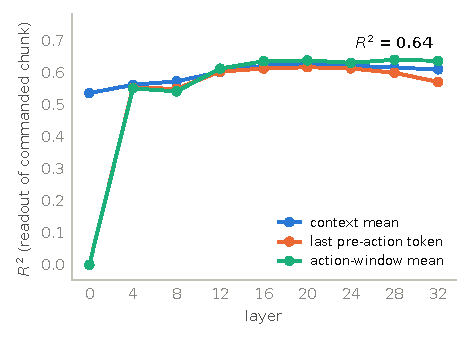
\includegraphics[width=\columnwidth]{fig_e1.pdf}
\caption{The commanded 56-dim chunk is linearly readable from the
pre-action state $h(t)$ (5-fold CV $R^2$; plateau $0.62$--$0.64$ at layers
16--28; the two layer-0 pools at $R^2\!\approx\!0$ are structurally
degenerate). The plan is \emph{present}---and its best readout cell
replicates exactly (L28/action-window mean, $0.639\to0.638$)---but it is
not \emph{usable} for attribution.}
\label{fig:e1}
\end{figure}

\begin{takeaway}
Across two seeds, four suites, and two probe families, the world-model
account holds for \emph{content} (the motor plan is present, stably placed)
and fails for \emph{use} (no readable self-vs.-external attribution), while
the same MLP family proves the comparison itself is cheap on raw
ingredients. Where probes do rise above floor, an observables-only control
rises at least as high---the states see the outcome; nothing in them owns
the action.
\end{takeaway}

\section{Results II: Novelty-Gated Compensation}
\label{sec:results-novelty}

\begin{figure}[t]
\centering
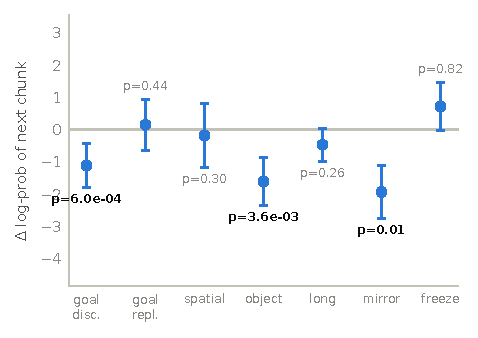
\includegraphics[width=\columnwidth]{fig_e3_logprob.pdf}
\caption{Log-probability arm of the behavioral fingerprint across all seven
runs: paired difference (hijack $-$ phase-matched self) in next-call
chosen-chunk log-probability. Points: pair-level means; error bars:
$\pm1$\,SE across episodes (the Wilcoxon unit); bold $p$: significant.}
\label{fig:e3lp}
\end{figure}

If the policy compared outcomes to commands, surprise should peak for
\textsc{freeze}, whose mismatch is the most decodable in the whole study
(P2r $0.886$ linear, $0.911$ MLP). The opposite happens
(\cref{fig:headline}b, \cref{fig:e3lp}).

\paragraph{The two poles, now powered.} After \textsc{mirror}---visibly
reversed motion---the next call's entropy rises $+0.014$ and chosen-chunk
log-probability falls $-1.94$ (episode-level $p{=}0.016$ and $0.012$,
$n{=}119$ episodes): the trend that was underpowered at $n{=}44$ in the
discovery wave reached significance exactly as the pre-registered expansion
asked. After \textsc{freeze}---a perfectly familiar, merely stationary
scene---nothing: $-0.004$ ($p{=}0.96$) and $+0.71$ ($p{=}0.82$) at
$n{=}115$, both point estimates on the wrong side, replicating the
discovery-wave null at $2.7\times$ the sample. Reaction tracks the visual
novelty of the outcome; mechanical decodability, which orders the arms the
other way, predicts none of it.

\paragraph{Swap reactions are real but fragile---and we report that.} In
the discovery run, \textsc{swap} produced a clear reaction ($+0.010$
entropy, $-1.12$ log-prob; $p{=}2.4\times10^{-3}$, $6.0\times10^{-4}$;
$n{=}217$). It did \emph{not} replicate in the pre-registered fresh-seed
run ($+0.001$, $p{=}0.53$; $+0.14$, $p{=}0.44$; $n{=}149$)---same suite,
same protocol, same temperature---and across all five swap runs the score
is 2 of 5 significant (discovery goal; Object at $+0.013$/$-1.62$,
$p{=}0.011$/$3.6\times10^{-3}$), with Spatial and Long null. This is
consistent with the gating account---a same-task donor chunk is the least
visually novel intervention we run, so its effect sits at the detection
threshold and surfaces only in some seeds and suites---but the honest
summary is that the swap-level reaction is small ($\leq{+}0.013$ nats) and
inconsistently detected, and the behavioral half of our story now rests on
the well-powered \textsc{mirror}/\textsc{freeze} contrast, not on swap
$p$-values.

\paragraph{Compensation is partial.} Hijack-carrying episodes succeed less
often than clean ones---modestly under \textsc{swap} ($0.39$ vs.\ $0.51$
replication; $0.41$ vs.\ $0.46$ discovery), severely under \textsc{mirror}
($0.19$ vs.\ $0.45$) and on the long-horizon suite ($0.04$ vs.\ $0.22$).
And the correction itself is visible in commands: after \textsc{freeze},
the next command re-asserts the blocked motion beyond what command
autocorrelation predicts (innovation-corrected undo-alignment $0.47$ vs.\
$0.22$ \textsc{self} baseline, discovery wave). Visual feedback control
explains all of this with no efference required.

\begin{takeaway}
\emph{Novelty-gated compensation}: the policy corrects perturbations and
its uncertainty rises after them, but the gate is the visual unusualness of
the outcome---significant for \textsc{mirror} ($n{=}119$), absent for the
most mechanically blatant \textsc{freeze} ($n{=}115$), threshold-level for
stealthy \textsc{swap}s (2/5 runs). Compensation without encoding
\citep{ye2026prediction} survives the jump from minimal agents to 7B
policies, and acquires a concrete gating variable.
\end{takeaway}

\section{Pre-Registration Receipts, and the Next Comparison}
\label{sec:receipts}

Interpretability nulls invite two failure modes: quietly re-running until a
positive appears, and quietly narrowing claims until the null is safe. Our
defense is procedural: wave 2's configurations and four readout rules were
committed to an append-only log before collection, and every verdict is
reported (\cref{tab:receipts})---including rule (c), where the data went
against our wave-1 reading (the small-arm probe excursions did \emph{not}
shrink; the pre-specified C$_{\Delta s}$ bound then localized them as
outcome perception, \cref{sec:results-visible}), and the swap-E3
non-replication, which demotes a wave-1 headline number.

\begin{table}[t]
\caption{Pre-registered readout rules (fixed before wave-2 data existed)
and verdicts.}
\label{tab:receipts}
\vskip 0.1in
\centering
\footnotesize
\begin{tabular}{p{0.44\columnwidth}p{0.44\columnwidth}}
\toprule
Rule (abridged) & Verdict \\
\midrule
(a) MLP P1/P3/P4 vs.\ MLP floor on the replication run; at floor $\Rightarrow$
claim strengthens beyond linear & at floor ($0.538$--$0.543$ vs.\ $0.532$);
claim strengthened \\
(b) Linear ladder replicates: floor and P2r within fold noise & yes
(\cref{tab:replication}) \\
(c) Do small-arm excursions shrink with $3\times$ data; does mirror E3 reach
significance at $n{\approx}130$? & excursions persist but are bounded by
C$_{\Delta s}$ (outcome perception); mirror E3 significant
($p{=}0.016$/$0.012$) \\
(d) Suites generalize only if P2r $\gg$ floor and rungs at floor
\emph{per suite} & holds per suite (linear $3/3$; MLP $1/1$ run) \\
--- (adverse) swap E3 in the replication run & did not replicate
($p{=}0.53$); swap claim demoted \\
\bottomrule
\end{tabular}
\vskip -0.1in
\end{table}

\textbf{The RL comparison (pre-registered, not yet run).} SFT never trains
the policy on the consequences of its own actions; on-policy RL does
precisely that \citep{shao2024deepseekmath,zhu2025wmpo}. The battery of
\cref{sec:protocol} applies unchanged to RL-post-trained sibling
checkpoints, and the outcomes are interpretable in both directions:
hidden-state probes separating from floor on the RL checkpoint would show
RL builds attribution-relevant representation SFT lacks (and the E3
fingerprint should migrate from novelty-gated toward mismatch-gated);
probes remaining at floor while compensation strengthens would show RL
sharpens the visual-servoing loop without new monitoring machinery. Either
way the question becomes a per-checkpoint measurement---which is the
protocol's point.

\section{How Naive Versions of This Experiment Return the Wrong Answer}
\label{sec:traps}

Most of our effort went into making the result interpretable rather than
into collection. Five pitfalls, each caught by a control now part of the
protocol:

\textbf{(T1) Best-cell selection inflates ladders.} P1's best cell beats
the fixed-cell permutation null in \emph{every} run (e.g.\ $0.543$ vs.\
$p_{95}{=}0.523$ in the replication)---naively ``above chance.'' Given the
same 27 tries, shuffled-label P0 reaches $0.536$--$0.542$. At pilot scale
($n{=}138$) the selection gap was $0.06$--$0.12$: small-$n$ probe sweeps
without a selection-matched null overclaim by construction.

\textbf{(T2) A linear ``oracle'' cannot compute agreement---and a nonlinear
one can.} Logistic regression on $a \oplus \Delta s$ is bilinear-blind; on
synthetic data with fully determined labels it scores $0.52$ where explicit
comparison features score $0.94$. Real data behaved as predicted per
transform (P2 at/below chance for mean-preserving \textsc{swap} in all five
runs; $0.587/0.561$ for \textsc{mirror}/\textsc{freeze}, which leak through
the marginal). The sequel matters as much: the \emph{same} concatenation
under a one-hidden-layer MLP recovers the comparison ($0.687$--$0.851$
across arms), which is what licenses reading the MLP's failure on
hidden-state features as absence of signal rather than weakness of family
(\cref{sec:results-cheap}). An acceptance gate on the linear concatenation
baseline would have misfired in both directions.

\textbf{(T3) Command autocorrelation fakes ``correction.''} The intuitive
undo-alignment metric reduces to $+\langle a_{\text{prev}},
a_{\text{next}}\rangle$ under \textsc{freeze}, so any smooth policy scores
as corrective: a provably open-loop simulation with $\rho{=}0.9$ scores
$+0.83$ raw and $0.00$ after AR(1) innovation correction. On real data
($\rho{=}0.63$--$0.72$) the raw metric inflates $2$--$4\times$.

\textbf{(T4) Task competence gates intervention strength.} On tasks the
policy cannot perform it barely moves and emits near-identical chunks across
episodes, making \textsc{swap} a near-no-op (first pilot: P2r $0.585$---the
oracle itself near chance). Three single-variable pilots isolated this;
competent tasks restore P2r to $0.749$ with controls at chance.

\textbf{(T5) Visible outcomes make any probe look like self-knowledge.}
In the gross-violation arms, hidden-state probes genuinely clear their
floors (up to $0.636$); without further controls this reads as ``the policy
knows it was hijacked.'' The observables-only control C$_{\Delta s}$
matches or exceeds every such excursion within-family, and C$_{\text{cmd}}$
stays at chance---the probes are reading the outcome's appearance, which
requires no access to the command at all. Any above-floor probing result on
intervention data needs an observables-only twin at the same probe family
before it can be read as internal attribution.

\begin{takeaway}
A probing null is only as meaningful as its nulls---and a probing
\emph{positive} is only as meaningful as its observables-only twin. T1--T5
are not specific to VLAs; any best-of-$N$ sweep, any concatenation
``oracle,'' any correction metric on autocorrelated actions, and any
intervention whose outcome is visible inherits them.
\end{takeaway}

\section{Limitations and Falsification Conditions}
\label{sec:limits}

\textbf{Probe reach.} ``Readable'' means: by linear probes and 256-unit
one-hidden-layer MLPs, on 27 layer$\times$pool \emph{pooled} summaries of
the residual stream, at $n{\approx}1.1$--$2.4$k. Deeper decoders, or
token-resolved features inside the 56-position action window, could in
principle read a code these summaries wash out. \emph{Falsifier:} any
decoder family separating from its own selection-matched floor on these
features (frozen features and code are released), or on token-level
captures.
\textbf{Dimensionality asymmetry.} The capacity argument compares an
outcome block of a few dozen simulator dimensions against 4096-dim pooled
states; at fixed $n$ a weak high-dimensional code is harder to extract than
a compact mechanical one. Two internal checks bound the concern---the same
MLP family does clear floors on 4096/8192-dim inputs when outcome
information is present (\cref{sec:results-visible}), and the detectability
window is quantified ($\approx0.03$--$0.04$ balanced accuracy above
floor)---but a code weaker than that window survives all of our probes.
\textbf{Swap-level behavior.} The swap E3 effect is small and was detected
in 2 of 5 runs, not in the pre-registered replication; we accordingly rest
no conclusion on it beyond ``at threshold.'' \emph{Falsifier for the
gating claim:} a transform matched in visual novelty to \textsc{mirror} but
with an \emph{intact} command--outcome link producing no reaction, or a
visually quiet transform producing one.
\textbf{Coverage.} Two pre-registered MLP passes (Object, Long) were cut by
a budgeted-compute rule and remain open; hidden states are retained. One
model family (OpenVLA-OFT variants), one simulator family (LIBERO), one
serving stack; rollouts capped at 320 steps (512 on Long).
\textbf{Phase structure.} Matched negatives sit a median of 2 calls earlier
than positives (structural); C$_{\text{ph}}$ ($0.486$--$0.533$ across runs
and families) bounds what phase alone explains, and the bias is
anti-conservative for positives, so the attribution null stands a fortiori.

\section{Conclusion}

Audited causally, 7B VLA policies compensate for hijacked actions through a
loop gated by visual novelty while exposing no readable trace---linear or
one-hidden-layer MLP---of their own agency: not on the discovery seed, not
on a pre-registered replication, not on three further suites with their own
checkpoints, even though the motor plan is stably decodable from the same
states and a 256-unit MLP computes the missing comparison outright when
handed the raw ingredients. Where probes do fire, an observables-only
control fires at least as hard: the states register how the world looks,
not who moved it. The Hijack--Probe protocol turns the
world-model-vs.-action-blind debate into per-checkpoint measurements at
under 5 GPU-hours per subject, and the standing pre-registered comparison
asks the next question: is self-attribution something post-training on
one's own consequences can buy?

\section*{Impact Statement}

This paper analyzes what a robot policy internally represents about its own
actions. Better tools for auditing self-attribution bear on the safe
deployment of embodied systems (does a policy notice being overridden?) and
on evaluating world-model claims. We release code, data, and the
pre-registration log for reproducibility; we do not foresee direct negative
societal impacts beyond those general to robot learning research.

\bibliography{refs}
\bibliographystyle{icml2026}

\appendix
\onecolumn

\section{Full Ladders per Run: Linear Family}
\label{app:ladders}

\begin{table}[h]
\caption{Linear-family ladders for all seven runs: balanced accuracy at each
probe's best layer$\times$pool cell ($\pm$ fold sd; single-cell probes P2,
P2r, and controls have no selection). Floors and permutation nulls computed
per run. Success rates are episode success in hijack-carrying vs.\ clean
episodes.}
\label{tab:arms-linear}
\vskip 0.1in
\centering
\scriptsize
\setlength{\tabcolsep}{2.5pt}
\begin{tabular}{lccccccc}
\toprule
& \shortstack{\textsc{swap} goal\\disc.} & \shortstack{\textsc{swap} goal\\repl.} & \shortstack{\textsc{swap}\\spatial} & \shortstack{\textsc{swap}\\object} & \shortstack{\textsc{swap}\\long} & \textsc{mirror} & \textsc{freeze} \\
$n$ (samples) & 1716 & 1266 & 1202 & 1478 & 2354 & 1226 & 1056 \\
\midrule
P0 floor & $0.536\pm0.011$ & $0.541\pm0.026$ & $0.533\pm0.026$ & $0.542\pm0.018$ & $0.523\pm0.014$ & $0.521\pm0.026$ & $0.538\pm0.040$ \\
perm.\ $p_{95}$ (fixed cell) & $0.516$ & $0.523$ & $0.532$ & $0.528$ & $0.521$ & $0.527$ & $0.529$ \\
P1 & $0.525\pm0.025$ & $0.543\pm0.035$ & $0.563\pm0.038$ & $0.566\pm0.026$ & $0.546\pm0.013$ & $0.567\pm0.028$ & $0.543\pm0.030$ \\
P3 & $0.525\pm0.019$ & $0.532\pm0.023$ & $0.567\pm0.036$ & $0.565\pm0.028$ & $0.545\pm0.014$ & $0.568\pm0.029$ & $0.565\pm0.017$ \\
P4 & $0.533\pm0.012$ & $0.536\pm0.011$ & $0.558\pm0.042$ & $0.576\pm0.022$ & $0.549\pm0.026$ & $0.597\pm0.011$ & $0.566\pm0.045$ \\
P2 (concat) & $0.494\pm0.044$ & $0.463\pm0.022$ & $0.500\pm0.015$ & $0.504\pm0.029$ & $0.502\pm0.026$ & $0.587\pm0.026$ & $0.561\pm0.033$ \\
\textbf{P2r (comparison)} & $\mathbf{0.690\pm0.044}$ & $\mathbf{0.711\pm0.038}$ & $\mathbf{0.757\pm0.021}$ & $\mathbf{0.800\pm0.023}$ & $\mathbf{0.774\pm0.018}$ & $\mathbf{0.857\pm0.036}$ & $\mathbf{0.886\pm0.035}$ \\
C$_{\text{cmd}}$ & $0.497$ & $0.475$ & $0.483$ & $0.512$ & $0.488$ & $0.515$ & $0.503$ \\
C$_{\Delta s}$ & $0.502$ & $0.488$ & $0.499$ & $0.513$ & $0.512$ & $0.623$ & $0.594$ \\
C$_{\text{phase}}$ & $0.486$ & $0.513$ & $0.514$ & $0.502$ & $0.521$ & $0.499$ & $0.505$ \\
success (hijack / clean ep.) & $0.41/0.46$ & $0.39/0.51$ & $0.44/0.58$ & $0.18/0.31$ & $0.04/0.22$ & $0.19/0.45$ & $0.40/0.32$ \\
\bottomrule
\end{tabular}
\end{table}

Cross-task transfer, discovery run (train on ${\sim}7$ tasks, test held-out):
P1 $0.505$, P3 $0.504$, P4 $0.501$. E1 readout: $R^2$ rising to a
$0.62$--$0.64$ plateau at layers 16--28; best cell layer~28/action-window
mean at $0.639$ (discovery) and $0.638$ (replication); regularization
interior to the search grid in 25/27 cells in both runs.

\section{Full Ladders: MLP Family}
\label{app:mlp}

\begin{table}[h]
\caption{MLP-family ladders (256-unit one-hidden-layer, \texttt{lbfgs};
selection-matched MLP floors). The Object and Long passes were cut by the
pre-registered compute budget; hidden states are retained on disk.}
\label{tab:arms-mlp}
\vskip 0.1in
\centering
\footnotesize
\begin{tabular}{lcccc}
\toprule
& \shortstack{\textsc{swap} goal\\replication} & \shortstack{\textsc{swap}\\spatial} & \textsc{mirror} & \textsc{freeze} \\
\midrule
P0 floor (MLP) & $0.532\pm0.029$ & $0.542\pm0.044$ & $0.532\pm0.025$ & $0.535\pm0.050$ \\
P1 & $0.538\pm0.026$ & $0.566\pm0.053$ & $0.581\pm0.038$ & $0.557\pm0.006$ \\
P3 & $0.540\pm0.017$ & $0.568\pm0.034$ & $0.577\pm0.030$ & $0.588\pm0.031$ \\
P4 & $0.543\pm0.013$ & $0.572\pm0.036$ & $0.612\pm0.022$ & $0.636\pm0.029$ \\
P2 (concat) & $0.687\pm0.016$ & $0.769\pm0.025$ & $0.851\pm0.020$ & $0.835\pm0.040$ \\
P2r (comparison) & $0.776\pm0.018$ & $0.827\pm0.020$ & $0.871\pm0.025$ & $0.911\pm0.036$ \\
C$_{\text{cmd}}$ & $0.499$ & $0.479$ & $0.520$ & $0.485$ \\
C$_{\Delta s}$ & $0.522$ & $0.607$ & $0.738$ & $0.825$ \\
C$_{\text{phase}}$ & $0.533$ & $0.527$ & $0.503$ & $0.498$ \\
\bottomrule
\end{tabular}
\end{table}

\section{Behavioral Fingerprint per Run}
\label{app:e3}

\begin{table}[h]
\caption{E3 across all runs: paired mean difference (hijack $-$
phase-matched self) in next-call entropy (nats) and chosen-chunk
log-probability; episode-level Wilcoxon $p$. The wave-1 task-matched row is
a re-analysis of the discovery run restricted to the five mirror/freeze
tasks, not an independent sample.}
\label{tab:e3}
\vskip 0.1in
\centering
\small
\begin{tabular}{lccccc}
\toprule
Run & $\Delta$entropy & $p$ & $\Delta$log-prob & $p$ & $n_{\text{ep}}$ (pairs) \\
\midrule
\textsc{swap} goal, discovery & $+0.010$ & $2.4\times10^{-3}$ & $-1.12$ & $6.0\times10^{-4}$ & 217 (858) \\
\quad task-matched subset & $+0.012$ & $4.5\times10^{-3}$ & $-1.38$ & $3.1\times10^{-3}$ & 120 (561) \\
\textsc{swap} goal, replication & $+0.001$ & $0.53$ & $+0.14$ & $0.44$ & 149 (633) \\
\textsc{swap} spatial & $+0.004$ & $0.26$ & $-0.19$ & $0.30$ & 138 (601) \\
\textsc{swap} object & $+0.013$ & $0.011$ & $-1.62$ & $3.6\times10^{-3}$ & 153 (739) \\
\textsc{swap} long & $+0.002$ & $0.43$ & $-0.47$ & $0.26$ & 123 (1177) \\
\textsc{mirror} (expanded) & $+0.014$ & $0.016$ & $-1.94$ & $0.012$ & 119 (613) \\
\textsc{freeze} (expanded) & $-0.004$ & $0.96$ & $+0.71$ & $0.82$ & 115 (528) \\
\bottomrule
\end{tabular}
\end{table}

\section{The Wave-1 Small Arms, for the Record}
\label{app:wave1arms}

The discovery wave included 50-episode \textsc{mirror}/\textsc{freeze} arms
($n{=}442/392$ samples) whose hidden-probe excursions (P1 $0.583/0.582$
against floors of $0.535\pm0.067$/$0.528\pm0.064$) we then read as
``within those arms' noisy floors.'' The pre-registered $3\times$ expansion
tested that reading and refuted it: the excursions are real
(\cref{tab:arms-linear,tab:arms-mlp}) and are explained by outcome
visibility, not attribution (\cref{sec:results-visible}). Wave-1 E3 for
these arms: mirror $+0.004$ ($p{=}0.45$) / $-1.66$ ($p{=}0.16$) at
$n{=}44$; freeze $-0.003$ ($p{=}0.65$) / $+0.27$ ($p{=}0.82$) at $n{=}42$.

\section{Qualitative Examples (Random, Not Cherry-Picked)}
\label{app:qual}

\begin{figure}[h]
\centering
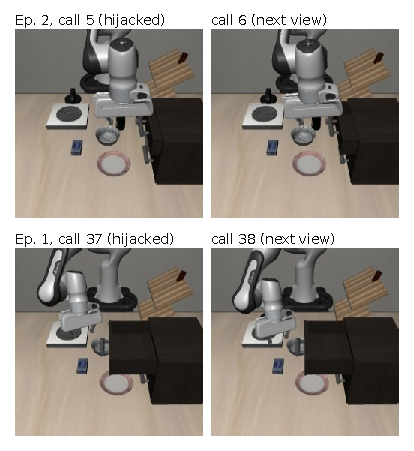
\includegraphics[width=0.42\textwidth]{fig_frames.pdf}
\caption{Two hijacked transitions drawn with a pre-registered seed from the
24 hijacks with saved frames in the task-3 pilot. \textbf{Top} (episode 2,
call 5): commanded net $\Delta y{+}5.7$, $\Delta z{-}4.4$, gripper channel
$+1$; executed $\Delta y{+}2.5$, $\Delta z{-}6.2$, gripper $-1$. The next
call became \emph{more} confident (entropy $0.091$ vs.\ episode self-mean
$0.240$; log-prob $-6.5$ vs.\ $-20.8$); the episode succeeds.
\textbf{Bottom} (episode 1, call 37): commanded up ($\Delta z{+}2.4$),
executed down ($-5.0$); entropy $0.409$ vs.\ $0.283$, log-prob $-32.0$ vs.\
$-26.7$; the episode fails. One of two random draws goes against the
population trend: within-episode scatter (entropy sd ${\approx}0.10$)
dwarfs the $+0.010$ mean shift, which is why a real distributional effect
coexists with floor-level per-instance decodability.}
\label{fig:frames}
\end{figure}

\end{document}
